\subsection{Editor Extension Components}

This section will describe the most relevant components, libraries or widgets for \acrshort{emf} in the \gls{cloud}, which can be used to create editor extensions.


\subsubsection{Sprotty}
Eclipse Sprotty is an \gls{open source}\footnote{Sprotty source: \href{https://github.com/eclipse/sprotty}{https://github.com/eclipse/sprotty}.} library to render diagrams in web browsers.
It uses Typescript, CSS and svg.
Sprotty can animate diagram changes.
The architecture is made with \gls{LSP} in mind, and supports having diagram data sent from a backend.
The library is configurable using dependency injection, and allows for adding custom nodes, edges and behaviors.
It also provides ``glue code'' for easy integration with \gls{LSP}, \gls{Theia} and \gls{ELK}.~\cite{smithEclipseSprotty2018}
An example of a sprotty diagram is shown in \cref{fig:sprotty-example}.

The library is mainly developed by TypeFox and EclipseSource, and managed by the Eclipse Foundation.~\cite{eclipsefoundationEclipseSprotty}

\begin{figure}[htbp]  % order of priority: h here, t top, b bottom, p page
  \centering
  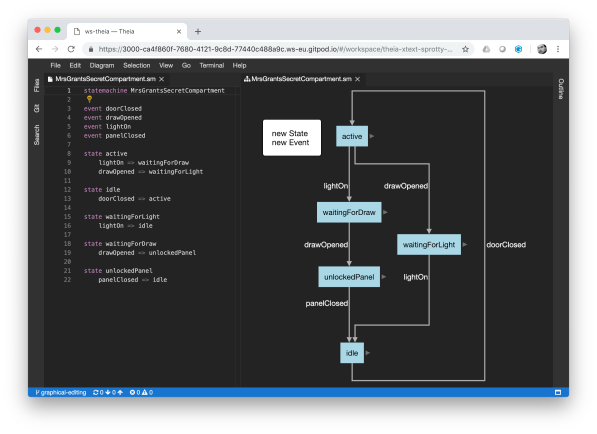
\includegraphics[width=.5\textwidth]{figures/sprotty-example.png}
  \caption[Sprotty Example]{This is a screenshot of Theia with a Sprotty diagram on the right side.~\cite{eclipsefoundationEclipseSprotty2020}}\label{fig:sprotty-example}
\end{figure}

\subsubsection{EMF.Cloud --- Theia Tree Editor}
The \emph{Theia Tree Editor} is an \gls{open source}\footnote{Theia Tree Editor source: \href{https://github.com/eclipse-emfcloud/theia-tree-editor/tree/master/theia-tree-editor}{https://github.com/eclipse-emfcloud/theia-tree-editor/tree/master/theia-tree-editor}.} framework for building tree editors in \gls{Theia}.~\cite{EclipseemfcloudTheiatreeeditor2020}
The framework is targeted to Theia Extensions (see \cref{sec:theia-extension}), and can not be used in \gls{VSCode}.
The main reason is the dependence on tree structures defined in the Theia \acrshort{IDE} project itself (see \cref{fig:theia-tree-editor-node}).
To render the property form, it uses the \emph{JSON-Forms} library (\cref{sec:json-forms}).
Additionally, it uses \gls{React}.

\begin{figure}[htbp]  % order of priority: h here, t top, b bottom, p page
  \centering
  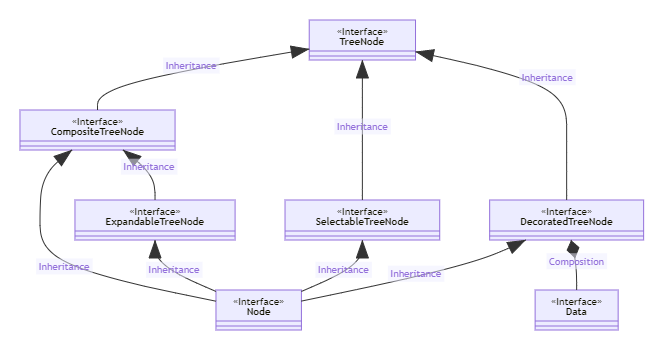
\includegraphics[width=\textwidth]{figures/theia-tree-editor-node.png}
  \caption[Theia Tree Editor Node's Class Hierarchy]{The Node class in Theia Tree Editor inherits multiple interfaces, all from the Theia \texttt{core} extension. Only \texttt{Node} resides in the Theia Tree Editor library itself.}\label{fig:theia-tree-editor-node}
\end{figure}

\subsubsection{JSON-Forms}\label{sec:json-forms}
JSON-Forms is an \gls{open source}\footnote{JSON-Forms source: \href{https://github.com/eclipsesource/jsonforms}{https://github.com/eclipsesource/jsonforms}.} library by EclipseSource for creating HTML form editors.
A form is defined by two key elements: a \emph{data/JSON schema} and a \emph{UI schema}.
The \gls{JSON} schema defines the data types and validations for input.
The User Interface (UI) schema defines the visible \emph{form controls} (text fields, groups, labels) and binds them to a object property in the JSON schema.~\cite{eclipsesourceJSONForms}
For an example of how a form can look like, see \cref{fig:json-forms-example}.

A visual editor for JSON-Forms schemas exist at \href{https://github.com/eclipsesource/jsonforms-editor}{https://github.com/eclipsesource/jsonforms-editor}.

\begin{figure}[htbp]  % order of priority: h here, t top, b bottom, p page
  \centering
  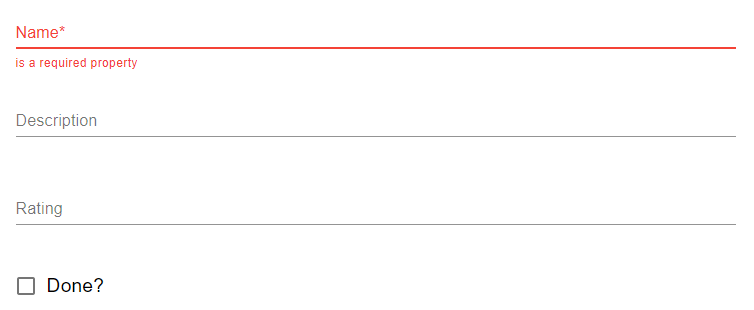
\includegraphics[width=.5\textwidth]{figures/json-forms-example}
  \caption[JSON-Forms Example]{An example of a form generated by JSON-Forms. It is displayed in a web browser.}\label{fig:json-forms-example}
\end{figure}

\subsubsection{EMF.Cloud --- Model Server}
% TODO: write
% https://github.com/eclipse-emfcloud/emfcloud-modelserver

\subsubsection{Eclipse Edit}
% TODO: write
% From genmodel. Strictly not cloud, but could aid a backend.

\subsubsection{EMF.Cloud --- emfjson-jackson}
% TODO: write
% https://github.com/eclipse-emfcloud/emfjson-jackson
% By emfjson aka @ghillairet, donated to emf.cloud

% ecore.js ?https://github.com/emfjson/ecore.js